% !TEX root = ./Cours.tex
\documentclass[../€Cours-complet/Cours-complet]{subfiles}

\titleorchapter{Fractions}{7}

\begin{document}

\maketitleCours

\section{L'écriture fractionnaire}

\begin{cours}[écriture fractionnaire]
	Soient a et b deux nombres, avec b non égal à 0. Le quotient de a par b est le nombre qui, multiplié par b, donne a.

	On peut le noter :
	\begin{itemize}
		\item a $÷$ b : c'est l'écriture \textbf{décimale}.
		\item $\dfrac{\text{a}}{\text{b}}$ : c'est l'écriture \textbf{fractionnaire}.

		      a est le \textbf{numérateur}.

		      b est le \textbf{dénominateur}.
	\end{itemize}
\end{cours}

\importantbox{
	On ne peut \textbf{jamais} diviser par 0.
}

\begin{exemple}
	Le quotient de 8 par 9 est $\dfrac{8}{9}$, et on a $\dfrac{8}{9} × 9 = 8$.
\end{exemple}

\begin{cours}[Fractions]
	Lorsque a et b sont des nombres \textit{entiers}, on dit que $\dfrac{\text{a}}{\text{b}}$ est une \textbf{fraction}.
\end{cours}

\section{Simplifier des fractions}

\begin{cours}
	Si on \textbf{multiplie} ou \textbf{divise} le numérateur \textbf{et} le dénominateur d'un quotient par le \textbf{même} nombre (différent de 0), la valeur du quotient reste la même.

	Si a, b, et k sont trois nombres, avec b ≠ 0 et k ≠ 0, alors

	$$ \dfrac{\text{a}}{\text{b}} = \dfrac{\text{a × k}}{\text{b × k}} = \dfrac{\text{a }÷\text{ k}}{\text{b }÷\text{ k}} $$
\end{cours}

\begin{exemple}
	\begin{align*}
		\dfrac{24}{30} & = \dfrac{24 ÷ 6}{30 ÷ 6} = \dfrac{4}{5}  &
		\dfrac{3,5}{6} & = \dfrac{3,5 × 2}{6 × 2} = \dfrac{7}{12}
	\end{align*}
\end{exemple}

\begin{cours}
	Pour \textbf{simplifier} une fraction, il faut écrire une autre fraction qui lui est égale, mais dont le numérateur et le dénominateur sont plus petits.

	Pour simplifier au \textit{maximum} une fraction, il faut utiliser le \textit{PGCD}, vu au chapitre 1. On dit alors que la fraction est \textbf{irréductible}.
\end{cours}

\begin{exemple}
	Pour simplifier $\dfrac{36}{15}$ :
	\begin{itemize}
		\item 36 et 15 sont divisible par 3.
		\item Donc on a $\dfrac{36}{15} = \dfrac{36 ÷ 3}{15 ÷ 3} = \dfrac{12}{5}$
	\end{itemize}
\end{exemple}

\begin{exemple}
	Pour simplifier $\dfrac{84}{70}$ :
	\begin{itemize}
		\item On a $84 = 2 × 2 × 3 × 7$ et $70 = 2 × 5 × 7$. Donc PGCD(84, 70) = 2 × 7 = 14.
		\item Donc on a $\dfrac{84}{70} = \dfrac{84 ÷ 14}{70 ÷ 14} = \dfrac{6}{5}$.
	\end{itemize}
\end{exemple}

\section{Comparaison de fractions}

\begin{cours}
	Pour placer une fraction $\dfrac{a}{b}$ sur une droite graduée, on peut :
	\begin{itemize}
		\item Calculer la valeur de $\dfrac{a}{b}$ ;
		\item Placer un point $A$ d'abscisse $a$, et diviser le segment $[OA]$ en $b$ partie égales.
	\end{itemize}
\end{cours}

\begin{exemple}
	Pour placer $\dfrac{6}{4}$, on peut:
	\begin{itemize}
		\item Calculer $\dfrac{6}{4} = 1,5$
		\item Placer le point $A$ d'abscisse 6, et diviser le segment $[OA]$ en 4 parties égales.
	\end{itemize}

	\vspace{0.7em}

	\begin{tikzpicture}
		\draw[->] (-0.2,0) -- (6.3,0);
		\foreach \x in {0,...,6} {
				\draw (\x,0) -- ++(0,-0.2) node[below] {\x};
			}
		\foreach \x in {1.5,3,4.5} {
				\draw[red] (\x,0.4) -- (\x,-0.4);
			}
		\node[red,above] at (1.5,0.4) {$\dfrac{6}{4}$};
		\node[red] at (6,0) {×};
		\node[red,above] at (6,0.1) {A};
	\end{tikzpicture}
\end{exemple}

\begin{cours}[Comparer des fraction]
	Pour comparer des fractions, il faut qu'elles aient le même \textbf{dénominateur}. On les compare alors par leur numérateur.
\end{cours}

\begin{exemple}
	$\dfrac{8}{5} < \dfrac{9}{5}$, car $8 < 9$.
\end{exemple}

\begin{methode}
	Si on veut comparer deux fractions qui n'ont pas le même dénominateur, il faut les modifier pour qu'elles aient le même dénominateur.

	Pour comparer $\dfrac{\text{a}}{\text{b}}$ et $\dfrac{\text{c}}{\text{d}}$ :

	On multiplie le numérateur et le dénominateur de $\dfrac{\text{a}}{\text{b}}$ par d, et le numérateur et le dénominateur de $\dfrac{\text{c}}{\text{d}}$ par b.

	\begin{center}
		\begin{tikzpicture}[node distance=0.7cm]
			\node (F1) {$\dfrac{\text{a}}{\text{b}} = \dfrac{\text{a×d}}{\text{\color{red}b×d}}$};
			\node[right=of F1] (ET) {et};
			\node[right=of ET] (F2) {$\dfrac{\text{c}}{\text{d}} = \dfrac{\text{c×b}}{\text{\color{red}d×b}}$};

			\node[below=of ET] {\color{red}b×d = d×b};
		\end{tikzpicture}
	\end{center}
\end{methode}

\begin{exemple}
	Si on veut comparer $\dfrac{12}{10}$ et $\dfrac{8}{6}$ :

	$$ \dfrac{12}{10} = \dfrac{12 × 6}{10 × 6} = \dfrac{72}{60} \hspace{1em}\text{ et }\hspace{1em} \dfrac{8}{6} = \dfrac{8 × 10}{6 × 10} = \dfrac{80}{60} $$

	Donc $\dfrac{12}{10} < \dfrac{8}{6}$.
\end{exemple}

\newpage

\section*{Avancé}

\begin{methode}[Comparer des fractions]
	Pour comparer deux fractions $\dfrac{a}{b}$ et $\dfrac{c}{d}$, on peut mettre le dénominateur de ces fractions au \textbf{PPCM} de $c$ et $d$.
\end{methode}

\begin{exemple}
	On voudrait comparer $\dfrac{17}{90}$ et $\dfrac{19}{110}$.
	\begin{itemize}
		\item 90 = 2×5×11 et 110 = 2×3×3×5, donc

		      PPCM(90, 110) = 2×3×3×5×11 = 990.
		\item On a 90 × 11 = 990 et 110 × 9 = 990. Donc

		      $$ \dfrac{17}{90} = \dfrac{17 × 11}{90 × 11} = \dfrac{187}{990} $$
		      $$ \dfrac{19}{110} = \dfrac{19 × 9}{110 × 9} = \dfrac{171}{990} $$

		      Donc $\dfrac{17}{90} > \dfrac{19}{110}$.
	\end{itemize}
\end{exemple}

\end{document}